\documentclass[t,aspectratio=169]{beamer}
\usetheme[progressbar=frametitle]{metropolis}
\usefonttheme{professionalfonts}
\usepackage{appendixnumberbeamer}

\usepackage{booktabs}
\usepackage[scale=2]{ccicons}

\usepackage{graphics,graphicx,amssymb,amsmath,pgf,comment,hyperref}
%\usepackage[xcolor=pst]{pstricks}
\usepackage{array}
\usepackage{pgfshade}
\usepackage[round]{natbib}
\usepackage[absolute,overlay]{textpos}
\usepackage{pifont}
\usepackage{dcolumn}
\usepackage{textpos}
\usepackage{color}					
\usepackage{xcolor,colortbl}
\usepackage{tikz}
\usepackage{bbm}
\usepackage{curves}
\usepackage{mathtools}
\usepackage{times}
\usepackage{verbatim}
\usetikzlibrary{snakes,arrows,shapes,positioning}
\def\augie{\fontencoding{T1}\fontfamily{augie}\selectfont}

\usepackage{pgfplots}
\usepgfplotslibrary{dateplot}

\usepackage{xspace}
\newcommand{\themename}{\textbf{\textsc{metropolis}}\xspace}

\setbeamertemplate{caption}{\raggedright\insertcaption\par}
\usetikzlibrary{calc,decorations.pathmorphing,patterns}
\pgfdeclaredecoration{penciline}{initial}{
    \state{initial}[width=+\pgfdecoratedinputsegmentremainingdistance,
    auto corner on length=1mm,]{
        \pgfpathcurveto%
        {% From
            \pgfqpoint{\pgfdecoratedinputsegmentremainingdistance}
                      {\pgfdecorationsegmentamplitude}
        }
        {%  Control 1
        \pgfmathrand
        \pgfpointadd{\pgfqpoint{\pgfdecoratedinputsegmentremainingdistance}{0pt}}
                    {\pgfqpoint{-\pgfdecorationsegmentaspect
                     \pgfdecoratedinputsegmentremainingdistance}%
                               {\pgfmathresult\pgfdecorationsegmentamplitude}
                    }
        }
        {%TO
        \pgfpointadd{\pgfpointdecoratedinputsegmentlast}{\pgfpoint{1pt}{1pt}}
        }
    }
    \state{final}{}
}


\title{Physician Behaviors and Hospital Influence}
\date{}
\author{Haizhen Lin \& \textbf{Ian McCarthy} \& Michael Richards}
\institute{April 20, 2019}

\begin{document}
\tikzstyle{every picture}+=[remember picture]
\everymath{\displaystyle}

\maketitle

\section{Background}

\begin{frame}{Physician Agency}
    \only<1>{
        Physician with decision-making authority for treatment
        \begin{itemize}
            \item Information asymmetry
            \item Regulatory restrictions
        \end{itemize}
    }
    \only<2->{
        Differential financial incentives between physician and hospital
        \begin{itemize}
            \item More procedures $=$ more revenue, but location of procedure may matter to hospital
            \item Hospital wants less cost with fixed payment, but physician dictates resource use
            \item Hospital as residual claimant on billable physician services
        \end{itemize}
    }
    \onslide<3->{
        $\longrightarrow$ Incentives for hospitals to influence physicians \\
        \vspace{.25in}
    }
    \onslide<4->{
        \noindent Most direct way (arguably) is to purchase physician practice
    }
\end{frame}

\begin{frame}{Changing Physician Relationships}
    \only<1>{
        \begin{figure}
            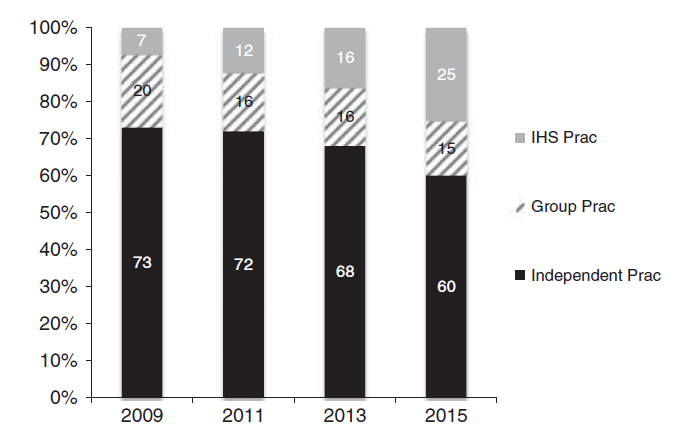
\includegraphics[height=2.4in,keepaspectratio]{Richardsetal.png}
            \caption{Richards \textit{et al.}, Medical Care, 2016}
        \end{figure}
    }
    \only<2>{
        \begin{figure}
            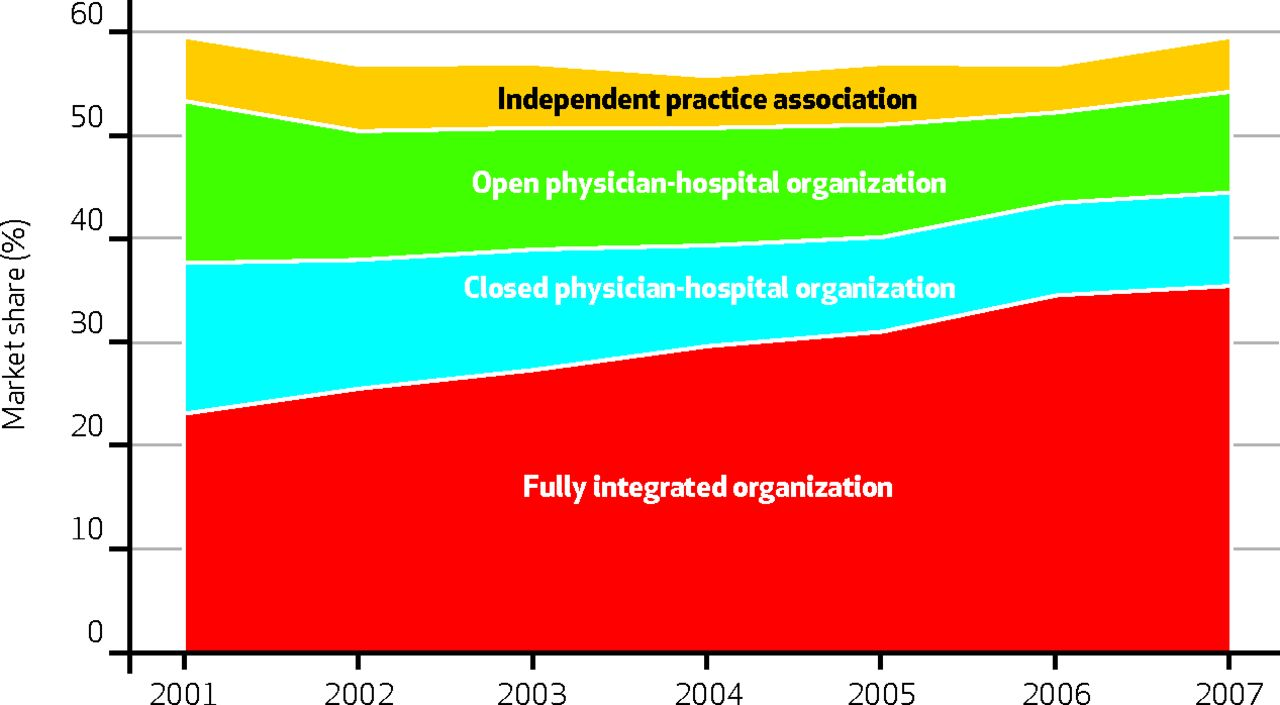
\includegraphics[height=2.3in,keepaspectratio]{Bakeretal.jpg}
            \caption{Baker, Bundorf, and Kessler, Health Affairs, 2014}
        \end{figure}
    }
\end{frame}

\begin{frame}{In context}
    \begin{itemize}
        \item Physician agency (Clemens \& Gottlieb 2014, AER; Afendulis \& Kessler 2007, AER; Gruber \& Owings 1996, RAND; Iizuka 2012, AER)
        \item Supply-side variation (Finkelstein \textit{et al.} 2016, QJE; Molitor 2018, AEJ: Policy)
        \item Vertical integration (Cuellar \& Gertler 2006, JHE; Ciliberto \& Dranove 2006, JHE; Baker \textit{et al.} 2016, JHE; Koch \textit{et al.} 2017, JHE)
    \end{itemize}
\end{frame}

\section{Theoretical Framework}
\begin{frame}{Physician Agency}
    \tikzstyle{na} = [baseline=-.5ex]
    \only<1->{
        Observed care at time $t$ is
        \begin{equation*}
            y_{ijk} = \arg \max_{y}  \theta_{u} \tilde{u} \left(y; \Gamma_{k}, \Gamma_{j}, \kappa_{i} \right) + \theta_{\pi} \pi \left(y; \Gamma_{k}, \Gamma_{j}, \kappa_{i} \right).
        \end{equation*}
    }
    \only<2->{
        \noindent With assumptions on linearity and separability in patient preferences:
        \begin{equation*}
            y_{ijk} =
            \tikz[baseline]{
                \node[fill=blue!20,anchor=base] (t1)
                {$ \alpha_{i} + x_{i}\beta $};
            } +
            \tikz[baseline]{
                \node[fill=red!20, ellipse, anchor=base] (t2)
                {$\Gamma_{jk}$};
            } + \epsilon_{ijk}
        \end{equation*}
        \begin{itemize}[<+-| alert@+>]
            \item[]<3-> Patient Preferences
                \tikz[na] \node[coordinate] (n1) {};
            \item[]<4-> Physician and hospital characteristics
                \tikz[na] \node[coordinate] (n2) {};
        \end{itemize}

        \begin{tikzpicture}[overlay]
            \path[->]<3-> (n1) edge [bend right] (t1);
            \path[->]<4-> (n2) edge [out=0, in=-90] (t2);
        \end{tikzpicture}
    }
\end{frame}

\begin{frame}{Estimation Strategy}
    \tikzstyle{na} = [baseline=-.5ex]
    \only<1-3>{
        Suggests two-step estimation strategy:
        \begin{enumerate}
            \item<2-> Estimate $y_{ijk} = \alpha_{i} + x_{i}\beta + \Gamma_{jk} + \epsilon_{ijk}$ at patient level (separately by year). This isolates variation in care to physicians and hospitals (not patients).
            \item<3-> Estimate $\hat{\Gamma}_{jkt} = \gamma_{j} + \gamma_{k} + \tau_{t} + z_{jkt}\delta + \eta_{jkt}$ with physician-hospital panel. This further isolates variation to physician-hospital interaction.
        \end{enumerate}
    }
    \only<4>{
        \begin{itemize}
            \item Draws from ``match values'' in labor literature (Abowd \textit{et al.}, 2002; Card \textit{et al.}, 2013, QJE )
            \item Exploits variation across inpatient stays and splits the separation of match value into two steps
            \item Identifies effects on match value from within-physician variation across hospitals (e.g., patient movers in Finkelstein \textit{et al.}, 2016, QJE)
        \end{itemize}
    }
    \only<5-8>{
        Traditional ``match value'' approach:
        \begin{equation*}
            y_{ijk} = \alpha_{i} + x_{i}\beta +
            \tikz[baseline]{
                \node[fill=blue!20,anchor=base] (t1)
                {$\Gamma_{j}$};
            } +
            \tikz[baseline]{
                \node[fill=green!20,anchor=base] (t2)
                {$\Gamma_{k}$};
            } +
            \tikz[baseline]{
                \node[fill=red!20,ellipse,anchor=base] (t3)
                {$\Gamma_{jk}$};
            } +
            \epsilon_{ijk}
        \end{equation*}
        \begin{itemize}[<+-| alert@+>]
            \item[]<6-> Physician effect
                \tikz[na] \node[coordinate] (n1) {};
            \item[]<7-> Hospital effect
                \tikz[na] \node[coordinate] (n2) {};
            \item[]<8-> Physician-hospital match value
                \tikz[na] \node[coordinate] (n3) {};
        \end{itemize}

        \begin{tikzpicture}[overlay]
            \path[->]<6-> (n1) edge [bend right] (t1);
            \path[->]<7-> (n2) edge [out=10, in=-70] (t2);
            \path[->]<8-> (n3) edge [out=0, in=-90] (t3);
        \end{tikzpicture}
    }
    \only<9->{
        Our approach:
        \begin{equation*}
            y_{ijk} = \alpha_{i} + x_{i}\beta + \underbrace{
            \tikz[baseline]{
                \node[fill=blue!20,anchor=base] (t1)
                {$\Gamma_{jk}^{t}$};
            }}_{
            \tikz[baseline]{
                \node[fill=green!20,anchor=base] (t2)
                {$\Gamma_{j}$};
            } +
            \tikz[baseline]{
                \node[fill=red!20,anchor=base] (t3)
                {$\Gamma_{k}$};
            } +
            \tikz[baseline]{
                \node[fill=orange!20,ellipse,anchor=base] (t4)
                {$z_{jkt}\delta$};
            }} +
            \epsilon_{ijk}
        \end{equation*}
        \begin{itemize}[<+-| alert@+>]
            \item[]<10-> Physician, hospital, and match effect (jointly)
                \tikz[na] \node[coordinate] (n1) {};
            \item[]<11-> Physician effect
                \tikz[na] \node[coordinate] (n2) {};
            \item[]<12-> Hospital effect
                \tikz[na] \node[coordinate] (n3) {};
            \item[]<13-> Physician-hospital integration
                \tikz[na] \node[coordinate] (n4) {};
        \end{itemize}

        \begin{tikzpicture}[overlay]
            \path[->]<10-> (n1) edge [out=0, in=-90] (t1);
            \path[->]<11-> (n2) edge [out=10, in=-70] (t2);
            \path[->]<12-> (n3) edge [out=5, in=-80] (t3);
            \path[->]<13-> (n4) edge [out=0, in=-90] (t4);
        \end{tikzpicture}
    }
\end{frame}

\begin{frame}{Intuition}
    \begin{itemize}
        \item Hospital influence on physicians is an interaction effect
        \item Potential influence should be net of patient preference
    \end{itemize}
\end{frame}

\section{Data}
\begin{frame}{Data Sources}
    \begin{itemize}
        \item CMS: 100\% inpatient and institutional outpatient Medicare claims data (2008-2015)
        \item SK\&A: Hospital ownership of physician practices and practice characteristics
        \item AHA, HCRIS, POS: Hospital characteristics
        \item Annual IPPS Impact Files: Hospital cost-to-charge ratios (CCR)
        \item ACS: County-level demographics, education, income, and employment
    \end{itemize}
\end{frame}

\begin{frame}{Sample Construction}
    \begin{itemize}
        \item<1-> Planned inpatient stays (elective admissions initiated by a physician, clinic, or HMO referral) and outpatient procedures with observed NPI for the operating physician
        \item<2-> Drop physicians operating in hospitals more than 120 miles from primary office or outside of contiguous U.S.
        \item<3-> Drop physicians with NPIs not matched in the SK\&A data
        \item<4-> Drop lowest/highest 1\% of charges and patients $<$ 65 years old
    \end{itemize}
  \uncover<5->{ $\longrightarrow$ 518,398 unique observations at the physician/hospital/year \\
   $\longrightarrow$ 7.5mm inpatient stays (47\% of total) and 24mm outpatient procedures}
\end{frame}

\section{Preliminary Evidence}
\begin{frame}{Total Spending by Integration Status}
    \only<1>{
        Estimate and plot residual from:
        \begin{equation*}
            y_{jkt} = \beta x_{jt} + \delta z_{kt} + \lambda_{k} + \lambda_{j} + \lambda_{t} + \varepsilon_{jkt}
        \end{equation*}
    }
    \only<2>{
        \begin{figure}
            \centering
            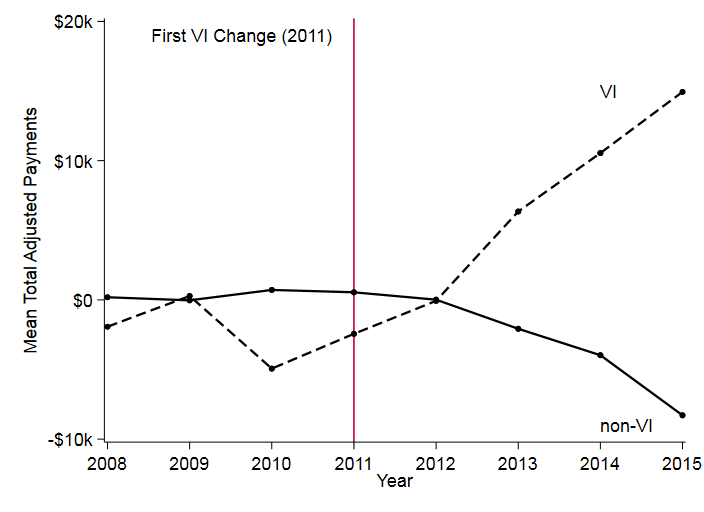
\includegraphics[height=2.5in,width=5in,keepaspectratio]{Summary_Pay3}
        \end{figure}
    }
    \only<3>{
        Components of aggregate effect:
        \begin{enumerate}
            \item Total number of patients for physician $k$
            \item Change in patient profile
            \item Reallocation of patients across hospitals
            \item Change in treatment for observationally equivalent patients
        \end{enumerate}
    }
\end{frame}


\section{Estimation of Match Values}
\begin{frame}{Specification}
    \only<1>{
    Two-step estimation strategy:
    \begin{enumerate}
        \item Estimate $y_{ijk} = \alpha_{i} + x_{i}\beta + \Gamma_{jk} + \epsilon_{ijk}$ at patient level (separately by year)
        \item Estimate $\hat{\Gamma}_{jkt} = \gamma_{j} + \gamma_{k} + \tau_{t} + z_{jkt}\delta + \eta_{jkt}$ with physician-hospital panel
    \end{enumerate}
    }
    \only<2>{
    \begin{equation*}
        y_{ijk} = \alpha_{i} + x_{i}\beta + \Gamma_{jk} + \epsilon_{ijk},
    \end{equation*}
    }
\end{frame}

\begin{frame}{Outcomes}
    \begin{equation*}
        \textcolor{red}{y_{ijk}} = \alpha_{i} + x_{i}\beta + \Gamma_{jk} + \epsilon_{ijk},
    \end{equation*}

    \begin{itemize}
        \item Total inpatient and outpatient Medicare payments
        \item Total inpatient and outpatient hospital costs (from cost-to-charge ratios)
    \end{itemize}
\end{frame}

\begin{frame}{Independent Variables}
    \begin{equation*}
        y_{ijk} = \textcolor{red}{\alpha_{i}} + x_{i}\beta + \Gamma_{jk} + \epsilon_{ijk},
    \end{equation*}

    \begin{itemize}
        \item Quartiles of total ``other'' Medicare payments and procedures
        \item Covers 2008 through 2015 period
        \item Beneficiary-specific ranking of health care utilization
    \end{itemize}
\end{frame}

\begin{frame}{Independent Variables}
    \begin{equation*}
        y_{ijk} = \alpha_{i} + \textcolor{red}{x_{i}}\beta + \Gamma_{jk} + \epsilon_{ijk},
    \end{equation*}

    \begin{itemize}
        \item Age, gender, race
        \item Indicators for ICD9 diagnosis code groups (18 diagnosis groups per variable plus missing group)
        \item Indicators for primary DRGs (with at least 1000 observations in a given year)
    \end{itemize}
\end{frame}

\section{Estimation of Hospital Influence}
\begin{frame}{Specification}
    \only<1>{
    Two-step estimation strategy:
    \begin{enumerate}
        \item Estimate $y_{ijk} = \alpha_{i} + x_{i}\beta + \Gamma_{jk} + \epsilon_{ijk}$ at patient level (separately by year)
        \item Estimate $\hat{\Gamma}_{jkt} = \gamma_{j} + \gamma_{k} + \tau_{t} + z_{jkt}\delta + \eta_{jkt}$ with physician-hospital panel
    \end{enumerate}
    }
    \only<2>{
    \begin{equation*}
        \hat{\Gamma}_{jkt} = \gamma_{j} + \gamma_{k} + \tau_{t} + z_{jkt}\delta + \eta_{jkt},
    \end{equation*}
    }
\end{frame}

\begin{frame}{Main Outcomes}
    \begin{equation*}
        \textcolor{red}{\hat{\Gamma}_{jkt}} = \gamma_{j} + \gamma_{k} + \tau_{t} + z_{jkt}\delta + \eta_{jkt},
    \end{equation*}

    \begin{table}[htb!]
    \centering
    \footnotesize
    \centerline{
    \begin{tabular}{l|rrrrr|r}
        & 2008  & 2012 & 2013 & 2014 & 2015 & Overall \\
        \hline
Total Payments &      7,152         &      8,171         &      8,501         &      8,941         &      9,169         &      8,094         \\
            &    (7,595)         &    (8,472)         &    (8,290)         &    (8,724)         &    (8,755)         &    (8,228)         \onslide<2->{\\
Total Costs &      9,387         &     11,323         &     11,756         &     12,237         &     12,736         &     10,965         \\
            &    (9,632)         &   (10,954)         &   (10,906)         &   (11,549)         &   (11,728)         &   (10,626)         }\\
    \end{tabular}}
    \end{table}

\end{frame}


\begin{frame}{Independent Variables}
    \begin{equation*}
        \hat{\Gamma}_{jkt} = \gamma_{j} + \gamma_{k} + \tau_{t} + \textcolor{red}{z_{jkt}}\delta + \eta_{jkt},
    \end{equation*}

    \begin{table}[htb!]
    \centering
    \footnotesize
    \centerline{
    \begin{tabular}{l|rrrrr|r}
        & 2008  & 2012 & 2013 & 2014 & 2015 & Overall \\
        \hline
Integrated       &       0.130         &       0.206         &       0.233         &       0.255         &       0.332         &       0.196         \\
                 &     (0.336)         &     (0.404)         &     (0.422)         &     (0.436)         &     (0.471)         &     (0.397)         \onslide<2->{\\
Physician FTE       &       24.23         &       28.59         &       31.14         &       31.74         &       33.13         &       28.43         \\
                    &     (99.28)         &     (109.8)         &     (120.5)         &     (120.0)         &     (119.5)         &     (110.9)         \onslide<3->{\\
Resident FTE        &       25.77         &       28.45         &       29.13         &       30.69         &       30.97         &       28.08         \\
                    &     (108.2)         &     (120.4)         &     (121.4)         &     (125.9)         &     (127.8)         &     (117.8)         \onslide<4->{\\
Nurse FTE           &       340.8         &       365.7         &       369.1         &       384.9         &       402.7         &       364.8         \\
                    &     (446.8)         &     (487.8)         &     (494.8)         &     (519.1)         &     (550.7)         &     (487.3)         \onslide<5->{\\
Other FTE           &       749.9         &       763.0         &       761.8         &       776.4         &       806.0         &       762.8         \\
                    &     (975.5)         &    (1032.4)         &    (1076.2)         &    (1101.5)         &    (1157.2)         &    (1037.4)         \onslide<6->{\\
Beds (100s)         &       1.980         &       1.967         &       1.958         &       1.982         &       2.009         &       1.976         \\
                    &     (2.160)         &     (2.142)         &     (2.137)         &     (2.172)         &     (2.235)         &     (2.154)         }}}}}\\
    \end{tabular}}
    \end{table}

\end{frame}

\begin{frame}{Independent Variables}
    \begin{equation*}
        \hat{\Gamma}_{jkt} = \gamma_{j} + \gamma_{k} + \tau_{t} + \textcolor{red}{z_{jkt}}\delta + \eta_{jkt},
    \end{equation*}

    \begin{table}[htb!]
    \centering
    \footnotesize
    \centerline{
    \begin{tabular}{l|rrrrr|r}
        & 2008  & 2012 & 2013 & 2014 & 2015 & Overall \\
        \hline
Practice Size&       13.73         &       17.31         &       17.31         &       17.82         &       18.41         &       16.10         \\
             &     (32.10)         &     (30.70)         &     (29.28)         &     (28.46)         &     (28.02)         &     (30.05)         \onslide<2->{\\
Experience   &       22.55         &       23.00         &       23.94         &       23.65         &       24.77         &       23.17         \\
             &     (6.496)         &     (6.703)         &     (6.950)         &     (6.902)         &     (6.989)         &     (6.746)         \onslide<3->{\\
\% Multi-Specialty &       0.249         &       0.248         &       0.266         &       0.284         &       0.344         &       0.264         \\
\% Surgery Center &       0.452         &       0.501         &       0.507         &       0.508         &       0.454         &       0.480         }}\\
    \end{tabular}}
    \end{table}

\end{frame}

\begin{frame}{Estimated Effects of Vertical Integration}
    \vspace{0.75in}
    \begin{table}[htb!]
    \centering
    \centerline{
    \begin{tabular}{l|rr}
        Outcome & Estimate & St. Error \\
        \hline\hline \onslide<2->{\vspace{-.1in}\\
        Total Medicare Payments & 75.121** & (30.902)  \onslide<3->{\\
        Total Hospital Costs & 132.466***  & (42.026) \onslide<4->{\\
        Total Stays          & 0.015*** & (0.004)   }}}\\
        \hline
        \multicolumn{3}{l}{\footnotesize * p-value $<$0.1, ** p-value $<$0.05, *** p-value $<$0.01}
    \end{tabular}}
    \end{table}
\end{frame}


\begin{frame}{Threats to Identification and Interpretation}
    Estimator is effectively a two-way fixed effects DD with time varying treatment
    \only<2>{
        \metroset{block=fill}
        \begin{block}{Potential Problems}
            \begin{enumerate}
                \item Vertical integration due to time-varying unobservables \& outcomes (standard DD concern)
                \item Weighted average of all 2$\times$2 DD estimates, with some potentially negative weights
            \end{enumerate}
        \end{block}
    }
\end{frame}

\begin{frame}{Event Study: Total Medicare Payments}
    \begin{figure}
        \centering
        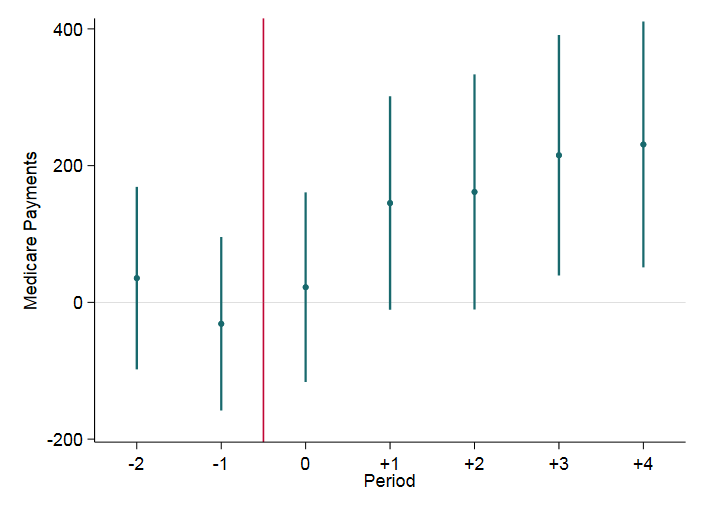
\includegraphics[height=2.5in,width=5in,keepaspectratio]{EventPay_All_2011}
    \end{figure}
\end{frame}

\begin{frame}{Event Study: Total Hospital (IP \& OP) Costs}
    \begin{figure}
        \centering
        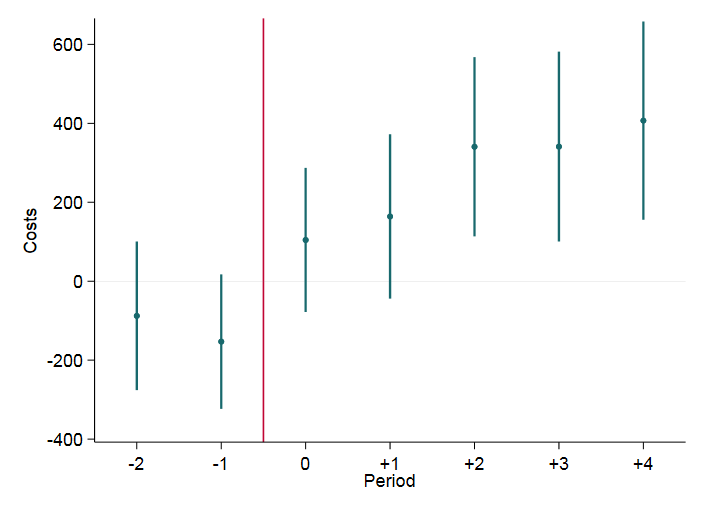
\includegraphics[height=2.5in,width=5in,keepaspectratio]{EventCharge_All_2011}
    \end{figure}
\end{frame}

\begin{frame}{Takeaways}
    \begin{itemize}
        \item Increase in payments and costs
        \item Evidence consistent with common trends assumption for total payments and costs
        \item Concerns about limited pre-period data
    \end{itemize}
\end{frame}


\begin{frame}{Endogeneity of physician-hospital integration}
    \label{ivs}
    \only<1>{
        Integration could be driven by:
        \begin{itemize}
            \item Unobserved, time-varying practice characteristics
            \item Existing costs and treatment patterns
        \end{itemize}
    }
    \only<2>{
        \metroset{block=fill}
        \begin{block}{1. Set of possible physician-hospital pairs}
            Form set of all hospitals where physician operates from 2008-2015
        \end{block}
    }
    \only<3>{
        \metroset{block=fill}
        \begin{block}{2. Estimate probability of integration}
            \begin{equation*}
                \text{Pr}\left(I_{jk}=1\right) = \frac{\text{exp}\left(\lambda z_{jk}\right)}{1+\text{exp}\left(\lambda z_{jk}\right)}
            \end{equation*}
            \vspace{-.3in}
            \begin{itemize}
                \item Hospital and practice characteristics
                \item Average differential distance (relative to nearest hospital in patient choice set)
                \item Differential distance interacted with hospital and practice characteristics
            \end{itemize}
        \end{block}
    }
    \only<4>{
        \metroset{block=fill}
        \begin{block}{2. Estimate probability of integration}
            \begin{equation*}
                \hat{\text{Pr}}\left(I_{jk}=1\right) = \frac{\text{exp}\left(\hat{\lambda} z_{jk}\right)}{1+\text{exp}\left(\hat{\lambda} z_{jk}\right)}
            \end{equation*}
            \noindent Intuition: Physicians less likely to seek/allow acquisition if patients live further away
        \end{block}
    }
    \only<5>{
        \metroset{block=fill}
        \begin{block}{2. Estimate probability of integration}
            \begin{equation*}
                \hat{\text{Pr}}\left(I_{jk}=1\right) = \frac{\text{exp}\left(\hat{\lambda} z_{jk}\right)}{1+\text{exp}\left(\hat{\lambda} z_{jk}\right)}
            \end{equation*}
            \noindent Intuition: Physicians less likely to seek/allow acquisition if patients live further away
        \end{block}
        \begin{equation*}
            \hat{\Gamma}_{jkt} = \gamma_{j} + \gamma_{k} + \tau_{t} + \underbrace{I_{jkt}}_{\mathclap{\hat{I}_{jkt}=\hat{\text{Pr}}(I_{jkt}=1)}} \delta_{1}  + \tilde{z}_{jkt}\delta_{2} + \eta_{jkt},
        \end{equation*}
    }
\end{frame}

\begin{frame}{IV Results: Aggregate Outcomes}
    \vspace{0.75in}
    \begin{table}[htb!]
    \centering
    \centerline{
    \begin{tabular}{l|rr}
        Outcome & Estimate & St. Error \\
        \hline\hline \onslide<2->{\vspace{-.1in}\\
        Total Medicare Payments & 870.384** & (340.409)  \onslide<3->{\\
        Total Hospital Costs & 2,545.815***  & (454.697) \onslide<4->{\\
        Total Stays          &  0.271*** & (0.042)   }}}\\
        \hline
        \multicolumn{3}{l}{\footnotesize * p-value $<$0.1, ** p-value $<$0.05, *** p-value $<$0.01}
    \end{tabular}}
    \end{table}
\end{frame}

\section{Does this Reflect Hospital Influence?}

\begin{frame}{Reallocation of Patients}
    \vspace{0.75in}
    \begin{table}[htb!]
    \centering
    \centerline{
    \begin{tabular}{l|rr}
        Outcome & Estimate & St. Error \\
        \hline\hline
        Total Medicare Payments & 75.121** & (30.902)  \\
        Total Hospital Costs & 132.466***  & (42.026) \\
        Total Stays          & 0.015*** & (0.004)   \onslide<2->{\\
        \hline
        Total Medicare Payments & 63.291** & (30.853) \\
        Total Hospital Costs & 124.830***  & (42.073) \\
        Total Stays          & 0.014**     & (0.004) } \\
        \hline
        \multicolumn{3}{l}{\footnotesize * p-value $<$0.1, ** p-value $<$0.05, *** p-value $<$0.01}
    \end{tabular}}
    \end{table}

\end{frame}

\begin{frame}{Areas with most incentives...}
    \only<1->{
        If hospital is residual claimant on billable procedures, should see more procedures within inpatient stays
    }
    \only<2>{
        \vspace{0.5in}
        \begin{table}[htb!]
        \centering
        \centerline{
        \begin{tabular}{l|rr}
            Outcome & Estimate & St. Error \\
            \hline\hline
            Inpatient Costs & 165.441*** & (50.165) \\
            Procedure Count & 0.030*** & (0.009) \\
            \hline
            \multicolumn{3}{l}{\footnotesize * p-value $<$0.1, ** p-value $<$0.05, *** p-value $<$0.01}
        \end{tabular}}
        \end{table}
    }
\end{frame}


\section{Effects on Total Procedures and Patients}
\begin{frame}{Aggregate Effects}
    Other ways integration posited to affect physician behavior:
    \begin{itemize}
        \item More procedures overall (largely coming from outpatient)
        \item Reallocating procedures (increased share to hospital)
        \item Changing patient profile (no evidence)
    \end{itemize}
\end{frame}

\begin{frame}{Summary of Results}
    \only<1>{
        \metroset{block=fill}
        \begin{block}{Main Findings}
            \begin{itemize}
                \item Increase in Medicare payments (\$75 to \$200) and hospital costs (\$130-\$350)
                \item Extrapolates to between \$55 and \$146 million in added Medicare payments from vertical integration
                \item Explains 4\% to 10\% of within-physician variation in Medicare payments
            \end{itemize}
        \end{block}
    }

    \only<2>{
        \metroset{block=fill}
        \begin{block}{Sensitivity}
           \begin{itemize}
                \item Event study consistent with common pre-trends but limited pre-period data
                \item IV results suggest conservative estimates
                \item No improvement in quality (mortality)
                \item As falsification test, no effects on payments or DRG weights per inpatient stay
            \end{itemize}
        \end{block}
    }

\end{frame}

\section*{Thank You!}


\end{document}






